\documentclass{article}
\usepackage{graphicx} % Required for inserting images
\usepackage{kotex}
\usepackage{subfigure}
\usepackage{caption}

\title{프로그래밍 언어 HW4}
\author{B811079 방병훈}
\date{20230523}

\begin{document}
\maketitle
\section{LISP에 대한 간단한 소개}
LISP은 LIST Programming의 약자로, 1958년 MIT에서 개발된 함수형 언어이다. 모든 자료는 연결 리스트로 처리하며, 컴파일 개념 없이 인터프리터 상에서 동작한다. 함수형 언어란 모든 연산 작업을 함수의 호출을 통해 수행하는 언어이다. Java에서 모든 변수가 하나의 객체이듯이, 함수형 언어는 모든 변수를 함수의 리턴으로 정의한다. 순차적 프로그래밍이나 OOP 이전에 등장한 개념이므로, 순차나 객체에 대한 개념은 가지고 있지 않다. 기능을 함수 단위로 구현함을 통해 빠르고 직관적으로 프로토타입을 만들 수 있다. 하지만 모든 연산을 함수 호출을 통해 처리하므로 연산 속도가 느리고 효율이 다소 떨어진다. 괄호의 사용도가 높고 명확한 표준이 존재하지 않아서 많은 방언이 만들어졌는데 이를 표준화한게 common lisp이다. 
\section{LISP 문법}
\subsection{기본 자료형 및 문법}
{\bf 기본 자료형}\\
Lisp를 구성하는 기초 블록은 아톰, 리스트, 문자열이다.  아톰은 숫자가 문자열 등의 다양한 데이터 구조가 동적 자료형으로 구성된 것이다. 리스트는 아톰이나 리스트를 구성 요소로 가진다. 즉, 리스트 자체는 재귀적으로 구성이 가능해서 데이터를 리스트의 구조로 표현할 수 있다. LISP에서 T는 참, nil은 거짓을 의미한다.\\
{\bf 기본 문법}\\
LISP는 모든 표기에 대해서 전위 표기를 사용한다. 예를 들어 (+1 3)의 결과는 4이다. 변수와 함수의 정의도 전위 표기를 따른다. 예를 들어 (setq x 10)은 x에 10을 저장한다는 것이고 (defun func (n))은 func라는 함수를 정의한다는 것이고 매개변수로 n을 받는다. setq 함수의 경우는 앞에 ‘를 붙이면 바로 뒤에 붙은 구문을 평가하지 않는다. (setq z ‘(+10 12)) 는 z에 (+10 12) 자체의 형태로 저장된다. 리스트의 선언은 list로 한다. (list 1 2 3 4 5)이라고 하면 리스트 1 2 3 4 5가 선언 된다. 리스트는 ‘를 활용해서 선언할 수 있다. (list 1 2 3 4 5)는 ‘(1 2 3 4 5)와 같다. 리스트 함수로는 car cdr cons가 있다. car은 리스트의 첫번째 원소를 반환하고 cdr은 첫번째 원소를 제외한 나머지 원소들로 이뤄진 리스트를 반환한다. cons는 첫번째 인수로 받은 원소를 리스트의 맨 앞에 삽입한 리스트를 반환한다. 주석의 경우 한줄 주석은  ;;, 줄의 일부만 주석으로 처리하려면 ""로 하면 된다. 
\newpage
{\bf 조건문}\\
조건문의 경우 COND가 있는데 COND는 c언어의 switch- case 구문과 매우 비슷하다. (COND (조건 1 실행 1) (조건 2 실행 2) … 이외 실행) 의 형식이다. 조건 1이 T(참)일경우 실행 1의 연산을 실행하고 조건들을 확인하다 맞는 조건이 없으면 이외를 실행한다. IF문도 마찬가지로 다른 언어의 if문과 동일하다. (IF 조건 실행1 실행2) 만약 조건이 참이면 실행1을 실행하고 조건이 거짓이면 실행 2를 실행한다.\\ 
{\bf 순차 수행문}\\
Common LISP에는 PROGN이라는 순차 수행문이 있다. (PROGN 실행1 실행2 … 실행n)인데 실행1부터 실행 n까지 수행하고 실행n의 결과값만 반환한다. \\
{\bf 출력 함수}\\
출력에는 print, prin1, princ, terpri, format이 있다. 우선 print의 경우 “”를 포함한 내용을 출력하고 ,개행문자를 무시하며 한줄의 공백과 한칸의 공백을 생성한다. princ의 경우 print와 기능이 같지만 “”를 제외한 결과가 출력된다. prin1의 경우 “”를 포함한 내용을 출력하지만 개행 문자를 무시한다. terpri의 경우는 한칸 띄우기라고 생각하면 된다. 문자열을 출력할때는 format을 사용하는데 첫번째 인자로는 t or nil, 두번째 인자로는 포맷팅 문자열, 그 이후로는 가변인자를 받는다. 첫번째 인자로 표준 입출력을 사용할지 말지를 정하고 두번째 포맷팅 문자열에는 ~로 시작하는 서식문자를 넣을 수 있다. ~A는 princ가 사용된것같이 인수가 출력된다, ~S는 prinl이 사용된것같이 인수가 출력되고, ~D는 정수인 인수가 10진수로 출력되고, ~F는 실수인 인수가 10진수 실수로 출력된다. ~C는 인수가 문자 출력으로 인쇄되고 ~\%는 새로운 줄이 출력된다. \\
{\bf let}\\
let은 새로운 지역 변수를 사용하는 표현식으로 두 부분으로 이루어져있다. 첫 번째는 변수를 생성하는 부분인데 (변수, 표현식)형태로 오게 되며 각 변수는 표현식으로 초기화된다. 이러한 변수들은 let의 범위 안에서만 유효하다. 두 번째 부분은 실행부분이다. 이 실행부분안에는 표현식이 여러개 들어갈 수 있고 마지막 표현식의 값이 let 전체의 최종 값으로 반환된다. \\
\subsection{내장 함수}
{\bf 간단한 함수들}\\
사칙연산을 위한 +-*/를 기본적으로 지원한다. RANDOM함수는 랜덤한 숫자를 반환하고 expt는 제곱을 반환한다. min, max 함수는 리스트 내의 최소,최대 값을 반환한다. abs는 절대값을 반환하고 sqrt는 루트값을 반환한다. sin cos tan은 각각 사인 코사인 탄젠트이고 round는 반올림을 지원한다. rem은 나머지를 반환한다. nth함수의 경우 리스트에서 특정 위치에 있는 원소를 반환하는 함수이다. parse-integer는 문자열을 정수로 변환하는 함수이다. readline함수는 사용자로부터 한 줄의 입력을 받는 함수이다. length는 리스트의 길이를 반환하는 함수이다. decf는 변수의 값을 1 감소시키는 매크로이다. 변수 값을 감소시킬 크기를 설정할 수 있지만 기본값은 1이다.\\
{\bf make-list}\\
make-list는 길이와 초기값을 정해서 리스트를 만들수 있다. 형식은 (make-list length : initial-element 초기값)이다. length는 리스트의 길이, initial-element는 초기값이다. 기본값은 nil이다.
\newpage
{\bf nth}\\
nth는 0부터 시작하는 인덱스로 원소에 접근한다. nth의 형식은 (nth i sequence)인데 i는 원소의 인덱스를 나타내는 정수값으로 0부터 시작하며, 원소에 접근하고자 하는 위치를 나타낸다. sequence는 리스트나 벡터이다. c언어에서 배열의 i번째값을 arr[i]로 접근하는 것처럼 common lisp는 (nth i arr) 이런 식으로 접근한다. nth는 시퀀스의 범위를 넘어가는 인덱스에 접근하면 nil을 반환한다.
\\{\bf loop}\\
loop는 반복문을 생성하는 매크로로 초기화, 종료조건, 반복문 내의 실행코드를 지정할 수 있다. loop의 구조는 (loop [initialization] [termination] [step-1] [step-2]… [return-form])이다. [initialization] 부분의 경우 반복문이 시작되기 전에 실행되는 초기화 코드로 변수를 초기화하거나 특정 코드를 실행할 수 있다. [termination]의 경우 반복문의 종료 조건을 지정할 수 있는 코드로 종료 조건이 만족되면 반복문이 종료된다. [step]은 반복문 내에서 실행되는 코드로 반복마다 수행되는 동작을 지정할 수 있다. 스텝은 여러 개를 지정할 수 있으며 순차적으로 실행된다. [result-form]은 반복문이 종료된 후에 평가되는 표현식이다. 이 표현식의 결과가 loop의 반환값이다. loop는 반복 키워드로 특정한 동작을 수행할 수 있다. \\
for는 변수의 초기값과 종료 조건을 지정해서 반복한다.  
\begin{verbatim}
(loop for i from 1 to 10 do 
	   (print i))
\end{verbatim}
위의 경우 i변수를 1부터 10까지 반복하면서 출력한다.  
\\while의 경우 주어진 조건이 참일때까지 반복한다. 
\begin{verbatim}
(loop while (> (random 10) 5) do 
	(print "Random number > 5"))
\end{verbatim}
이 코드의 경우 랜덤하게 생성된 숫자가 5보다 클 경우 반복한다.\\ 
unless는 주어진 조건이 거짓이 될 때 까지 반복한다.
\begin{verbatim}
(loop for i from 0 to 9
      unless (evenp i)
      do (print i))
\end{verbatim}
이 경우 i가 짝수가 아닐때만 실행코드를 수행한다. 
\\do는 반복문 내에서 수행할 코드의 블록을 지정한다.
\begin{verbatim}
(loop for i from 1 to 5 do
      (format t "Iteration ~a~%" i)
      (when (evenp i)
        (format t "Even number: ~a~%" i)))
\end{verbatim}
이 경우 1부터 5까지의 숫자를 반복하면서 각 숫자를 출력하고, 짝수인 경우에는 추가적인 메시지를 출력한다. 
\\collect는 반복 동작 중에 원하는 값을 수집하여 리스트나 배열로 반환한다.
\begin{verbatim}
(let ((evens (loop for i from 1 to 10
                   when (evenp i)
                   collect i)))
  (print evens))
\end{verbatim}
이 경우 1부터 10까지의 숫자 중에서 짝수인 숫자를 수집하고 evens 리스트에 저장한 후 출력한다.
\\when은 반복 중에 특정 조건이 참일 경우에만 실행 코드를 수행한다. when 키워드는 조건식과 실행 코드를 포함하고, 조건식이 참일 경우에만 실행 코드가 실행된다.
\begin{verbatim}
(loop for i from 1 to 10
      when (evenp i)
      do (print i))
\end{verbatim}
위의 경우 i가 짝수일때만 실행 코드를 수행한다. 

\section{코드}
\subsection{hw4a 코드}
\begin{verbatim}
;기본 아이디어는 한 열에는 퀸을 하나만 놓을 수 있다는 아이디어이다. 그리고 퀸이 이미 존재하는 열에는 퀸을 놓을 수 없다.
;따라서 열마다 퀸을 놓을 자리를 리스트로 만들면 행(칼럼)의 인덱스를 값으로 가진 일차원 배열로 퀸의 자리를 나타낼 수 있다.
;이후 퀸이 자리를 찾을 수 있는지 판단하는 함수를 구현한다. 그리고 자리를 찾을 수 없으면 거기까지만 탐색하고 
;찾을 수 있을때만 탐색을 진행한다. 즉, 첫번째 열부터 마지막 열까지 퀸이 들어갈 행을 일차원 리스트에 저장한다.

(format t "n-queen 문제입니다. n을 설정해주세요>>") ; n값을 입력받는다.
(let ((n (parse-integer (read-line)))) ; 입력받은 값을 정수로 변환해준후 n에 저장한다.
  (let ((row (make-list n :initial-element 0))) ; 퀸들의 위치를 저장하는 길이가 n인 리스트 생성하고 0으로 초기화한다. 
    (defun promising (x) ; 현재 열에서 유효한 위치인지 확인하는 함수이고, x는 현재 퀸이 배치된 열의 인덱스이다. 
      (loop for i from 0 below x  ;0~x-1까지는 퀸이 존재하므로 이러한 열들과 지금 고려하는 열이랑 충돌만 판단. 
            always (not (or (= (nth x row) (nth i row)) ; 같은 행에 위치한 퀸이 있는지 확인
                            (= (abs (- (nth x row) (nth i row))) (- x i)))))) ; 대각선에 위치한 퀸이 있는지 확인

    (defun nqueen (x)
      ; 퀸 배치 함수
      (if (= x n); 모든 퀸이 배치된 경우 즉, 탐색이 완료된 경우이다.
          (progn
            (print row) ; 해당 로우를 출력한다. 즉, n-queen 문제의 해답이다.
            (return-from nqueen)) ;nqueen 함수에서 탈출한다.
          (loop for i from 0 below n  ;아직 탐색중인 경우 반복문을 진행한다.
                do (progn             
                     (setf (nth x row) i) ; 현재 열에 퀸 배치한다. x는 열(칼럼) 값이다. 
                    ;즉, [x,i]에 퀸을 놓는다. 만약 성립 안하면 그 다음 i가 row[x]에 덮어씌워진다.리스트의 원소에 값을 할당하기 위해 setf를 사용했다.
                     (when (promising x) ; 유효한 위치인지 확인한다. 놓을 자리 있는지 판단하고 있으면 진행하고 없으면 다음 i로 넘어간다. 
                                         ;어차피 한 열에 한 자리만 가능하다. 따라서, 자리 찾으면 나가도 된다.
                       (nqueen (1+ x))))))) ;다음 열에 퀸 놓을자리 판단하러 진행한다.

    (nqueen 0) ; 퀸을 놓을 자리 탐색을 시작한다.
    ))
\end{verbatim}
\subsection{hw4a 코드 작동 방식}
저는 n-queen 문제를 이번 과제를 통해 처음 접했습니다. 그래서 lisp언어로 처음부터 작성하기에는 무리라고 판단하고 우선 python으로 구현했습니다. 파이썬 코드를 참고해서 필요한 함수들을 구글링을 통해 찾으면서 lisp로 n-queen 코드를 구현했습니다. n-queen 문제를 해결하는 방법은 많지만 저는 백트래킹 방식을 통해서 구현했습니다. 백트래킹 방식이란 정답을 찾아가는 도중에 정답이 아니라고 예상되거나 정답이 아닌경우 탐색을 중단하고 되돌아오는 방법입니다. 검색할 대상의 크기가 작을 경우 큰 차이가 없겠지만 대상의 크기가 커질수록 백트래킹 방식은 효율적입니다. n-queen 문제를 하나하나 확인하면서 계산을 한다면 계산은 지수시간이 걸려서 사실상 큰 n에서는 계산이 불가능합니다. 따라서, 실행시간을 단축하기 위해 백트래킹 방식을 사용했습니다. 제가 n-queen 문제를 해결한 기본 아이디어는 한 열에는 퀸을 하나만 놓을 수 있다는 것입니다. 또, 퀸이 존재하는 열에는 퀸을 놓을 수 없다는 것입니다. 따라서 열마다 퀸을 놓을 자리를 리스트로 만들면 행의 인덱스를 값으로 가진 일차원 리스트로 퀸의 자리를 나타낼 수 있습니다. 이후 퀸이 자리를 찾을 수 있는지 판단하는 함수를 구현하고 자리를 찾을 수 없으면 더 이상 탐색하지 않고 찾을 수 있을 때만 탐색하도록 했습니다. 프로그램이 종료되기 전에 함수는 첫번째 열부터 마지막 열까지 퀸이 들어갈 수 있는 행을 일차원 리스트로 반환합니다. promising이라는 함수는 해당 열에서 퀸이 들어갈 자리가 있는지 판단합니다. 만약 들어갈 자리가 없다면 nqueen 함수에서 더 이상 탐색을 진행하지 않고 돌아갑니다. nqueen 함수는 모든 퀸이 배치될때까지 반복하면서 퀸이 들어갈 자리를 탐색합니다. 끝까지 탐색을 진행하면 nqueen 함수의 리스트 row는 문제의 해입니다. 따라서 nqueen함수는 row를 출력하고 함수를 탈출합니다. 코드가 가독성이 안좋아서 코드 사진을 추가했습니다. 
\newpage
\begin{figure}[h]
    \centering
    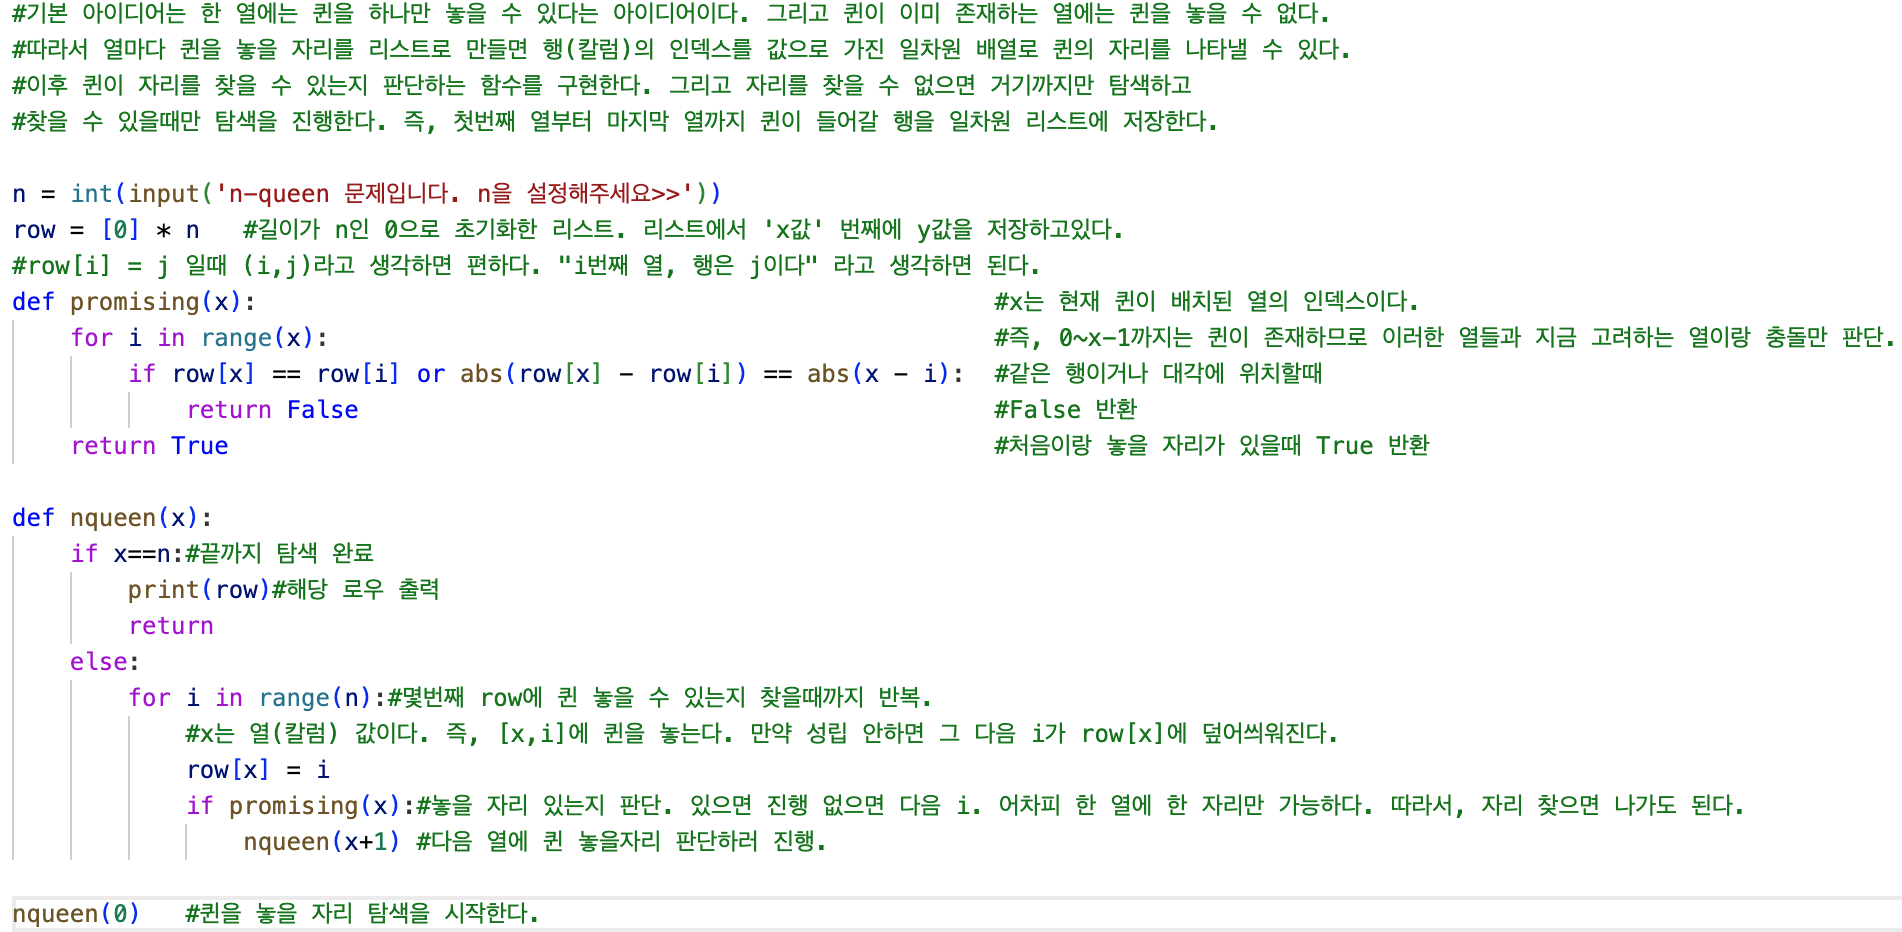
\includegraphics[width = 10cm]{nqueen_python.png}
    \caption{nqueen 문제 파이썬 코드}
    \label{fig:fig1}
\end{figure}
\begin{figure}[h]
    \centering
    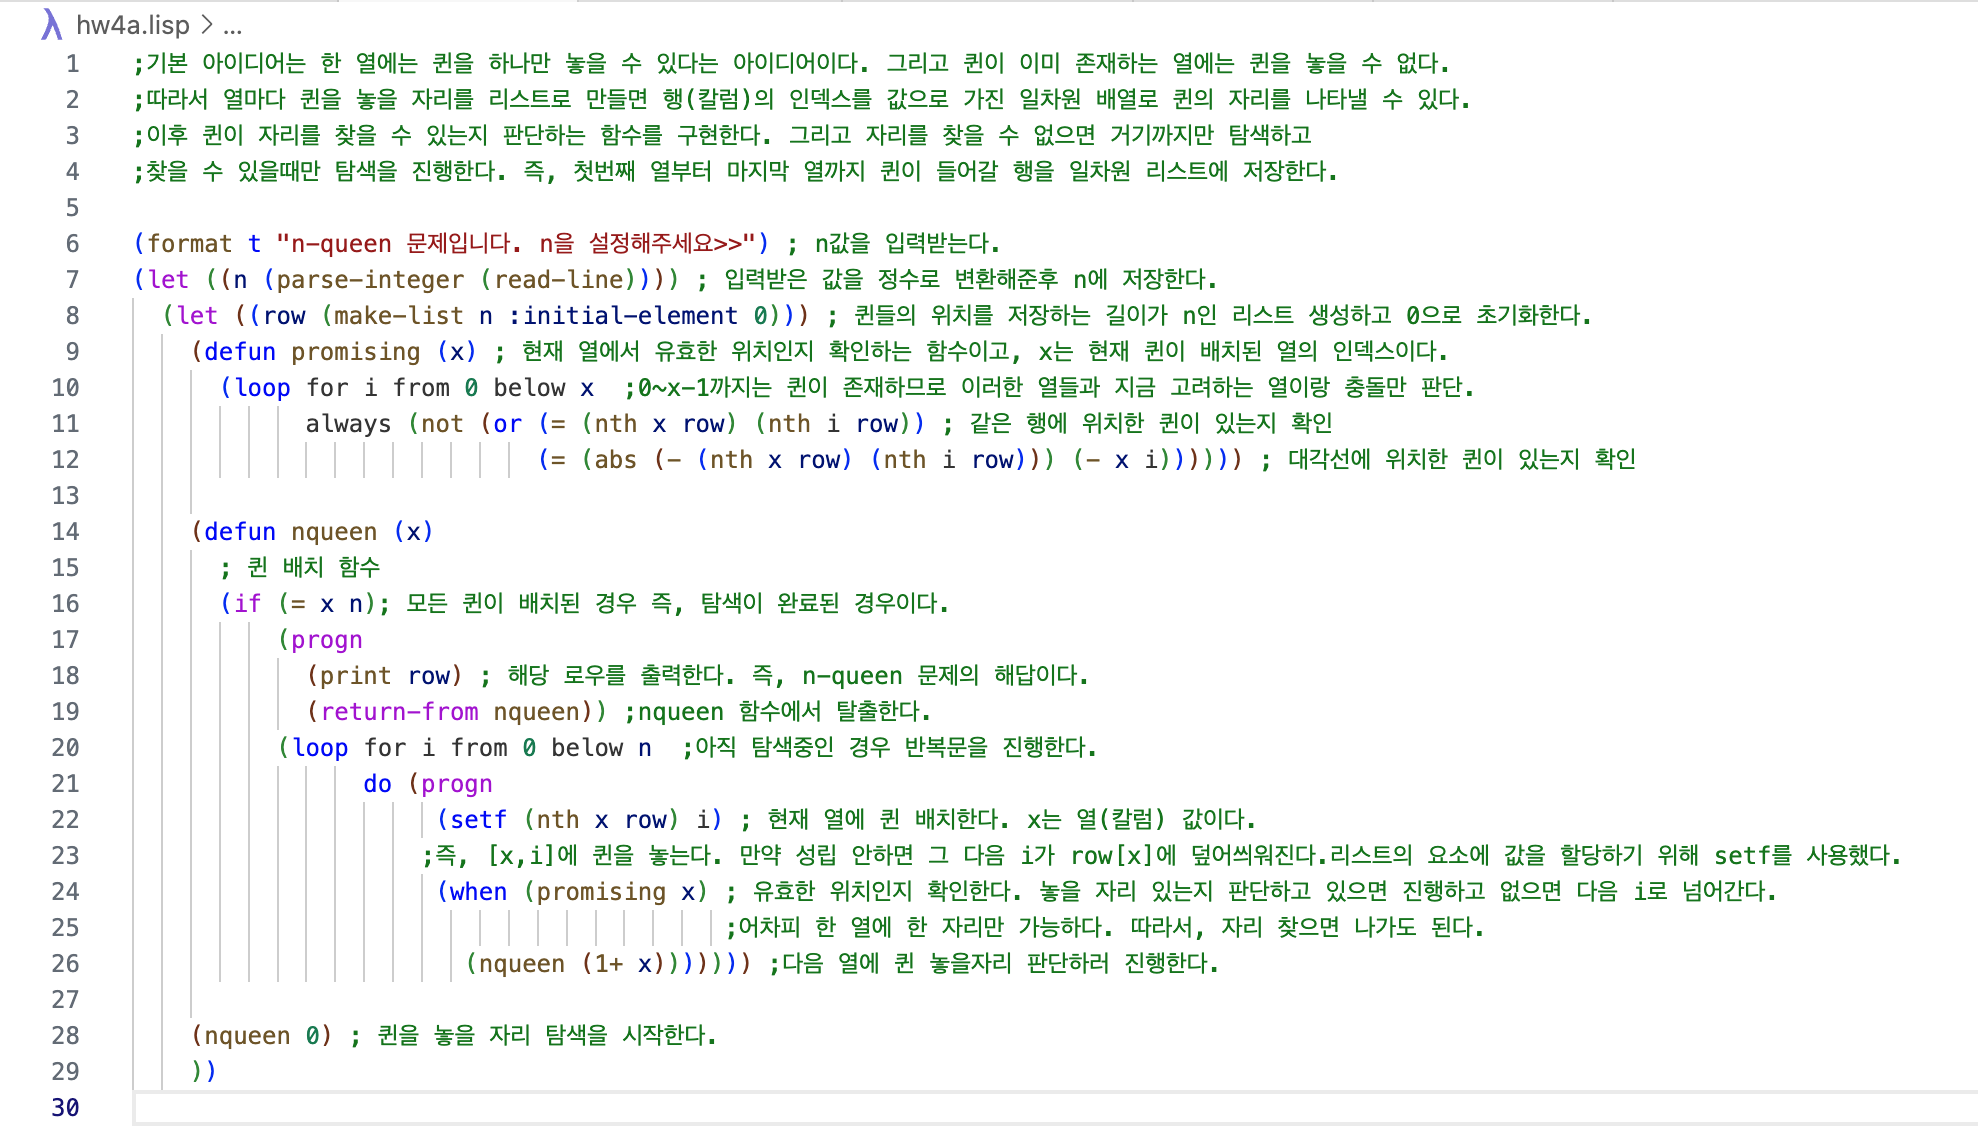
\includegraphics[width = 10cm]{hw4a_code.png}
    \caption{hw4a 코드}
    \label{fig:fig2}
\end{figure}
\begin{figure}[h]
    \centering
    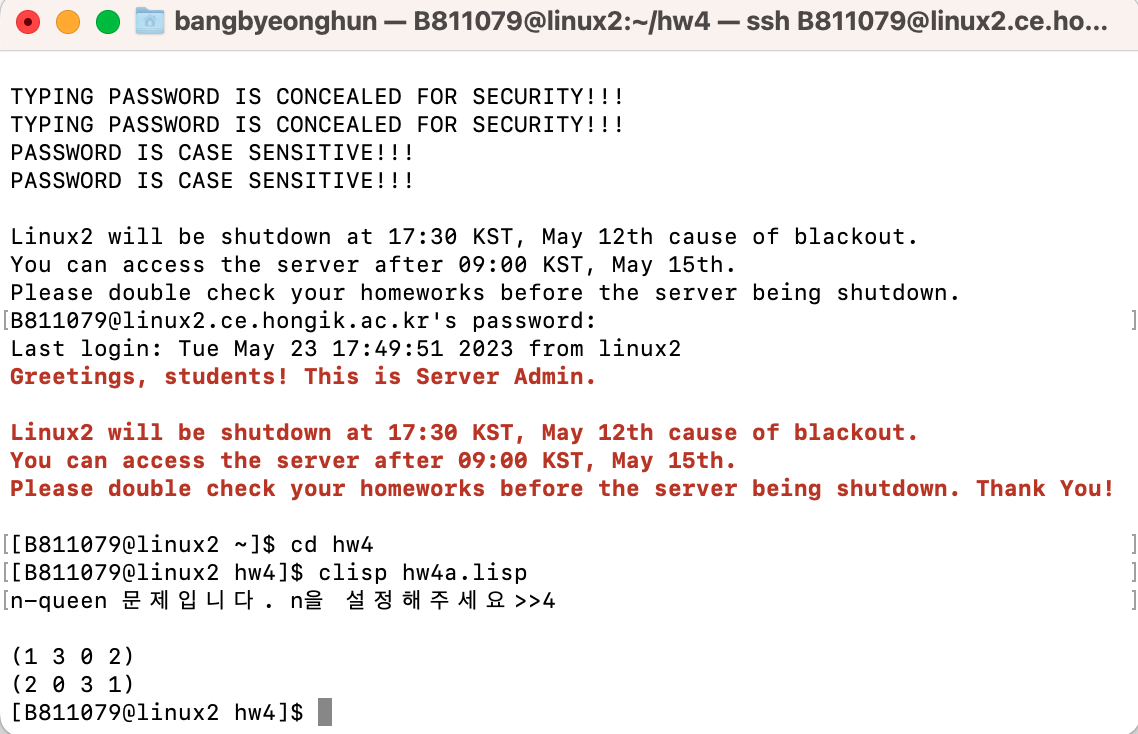
\includegraphics[width = 10cm]{hw4a_run.png}
    \caption{hw4a 실행결과}
    \label{fig:fig3}
\end{figure}
\newpage
\subsection{hw4b 코드}
\begin{verbatim}
(defun insort (arr) ;삽입정렬 함수이고 매개변수로 리스트를 받는다.
  (do ((i 1 (+ i 1)))  ; 인덱스 i는 1부터 시작하고 1씩 증가한다.
      ((>= i (length arr)))  ; i가 리스트의 길이를 초과하면 반복문을 종료한다.
    (let ((k (nth i arr))  ; k에 현재 인덱스의 원소를 저장한다. c언어로 치면 k = arr[i]
          (j (- i 1)))  ; j를 i의 이전 인덱스로 초기화한다.
      (loop
         (cond
          ((< j 0)  ; j가 0보다 작아지면 
           (setf (nth (+ j 1) arr) k)  ; k를 j+1번째 자리에 저장하고 arr[j+1] = k
           (return))  ; 반복문을 종료한다.
          ((< k (nth j arr))                  ; k가 j번째 원소보다 작으면(k < arr[j])
           (setf (nth (+ j 1) arr) (nth j arr))  ; j번째 원소를 j+1번째로 이동시킨다.
           (decf j))  ; j는 왼쪽으로 한칸 이동한다. (j--)
          (t  ; k가 j번째 원소보다 크거나 같으면(k>= arr[j])
           (setf (nth (+ j 1) arr) k)  ; k를 j+1번째 자리에 저장하고  arr[j+1] = k
           (return))))))  ; 반복문을 종료한다.
  arr)  ; 정렬된 리스트를 반환한다.

; 입력값을 리스트로 선언한다.
(setq TC1 '(11 33 23 45 13 25 8 135))
(setq TC2 '(83 72 65 54 47 33 29 11))

;테스트 케이스 리스트를 출력한다.
(print TC1)
(print TC2)
(terpri);개행한다.
;; insertionsort를 사용하여 정렬된 결과를 출력한다.
(format t "결과: ~a~%" (insort TC1))
(format t "결과: ~a~%" (insort TC2))
\end{verbatim}
\subsection{hw4b 코드 작동 방식}
Insertion sort(삽입정렬)란 리스트를 오름차순으로 정렬하는 방식중의 하나로(내림차순도 가능하지만 일반적으로 오름차순으로 정렬한다) 두 번째 자료부터 탐색을 시작해서 인덱스를 1씩 증가시키면서 리스트 상의 앞에 있는 자료들과 값을 비교해서 정렬하는 방식을 말합니다. 인덱스에 해당하는 값을 key값이라고 하면, key는 왼쪽 값들과 1대1로 비교를 하는데 만약 key가 왼쪽 값보다 크다면 인덱스가 1증가합니다. 하지만 key값이 왼쪽 값보다 작다면 해당 값을 한칸 오른쪽에 저장합니다. 이와 같은 과정을 반복하다 key값보다 작은 값을 만나면 그 값의 오른쪽 위치에 key값을 저장하고 인덱스를 1 증가시킵니다. key값보다 작은 값을 만나면 더 이상 비교하지 않고 저장하는 이유는 그 왼쪽 값들은 이미 정렬이 완료되어서 비교할 필요가 없기 때문입니다. 이러한 삽입 정렬을 구현하기 위해 저는 insort라는 함수를 만들었습니다. insort 함수는 리스트를 매개변수로 받아서 정렬하는 함수입니다. 처음 인덱스 i는 0부터 [리스트의 길이-1]까지 증가합니다. 만약 [i = 리스트의 길이]가 되면 반복문은 종료됩니다. k에 현재 인덱스의 원소(위에서 Key값)를 저장하고 리스트의 원소들과 비교를 합니다. j는 [i-1]부터 비교를 시작한다. 비교를 했을때 j번째 원소보다 작으면 j번째 원소를 한칸 오른쪽에 저장하고 j는 왼쪽으로 한칸 이동한다(1 감소한다). 비교를 하다 k가 j번째 원소보다 크거나 같으면 k를 j+1번째 자리에 저장하고 반복문을 종료한다. 만약 j가 0보다 작아지면 k를 j+1번째 자리에 저장하고 반복문을 종료한다. 이와 같은 과정을 리스트의 마지막 값까지 비교할 때까지 반복한다.
이후 테스트 케이스를 각각 TC1과 TC2라는 리스트로 저장해서 삽입정렬을 수행했다.

\newpage
\begin{figure}[h]
    \centering
    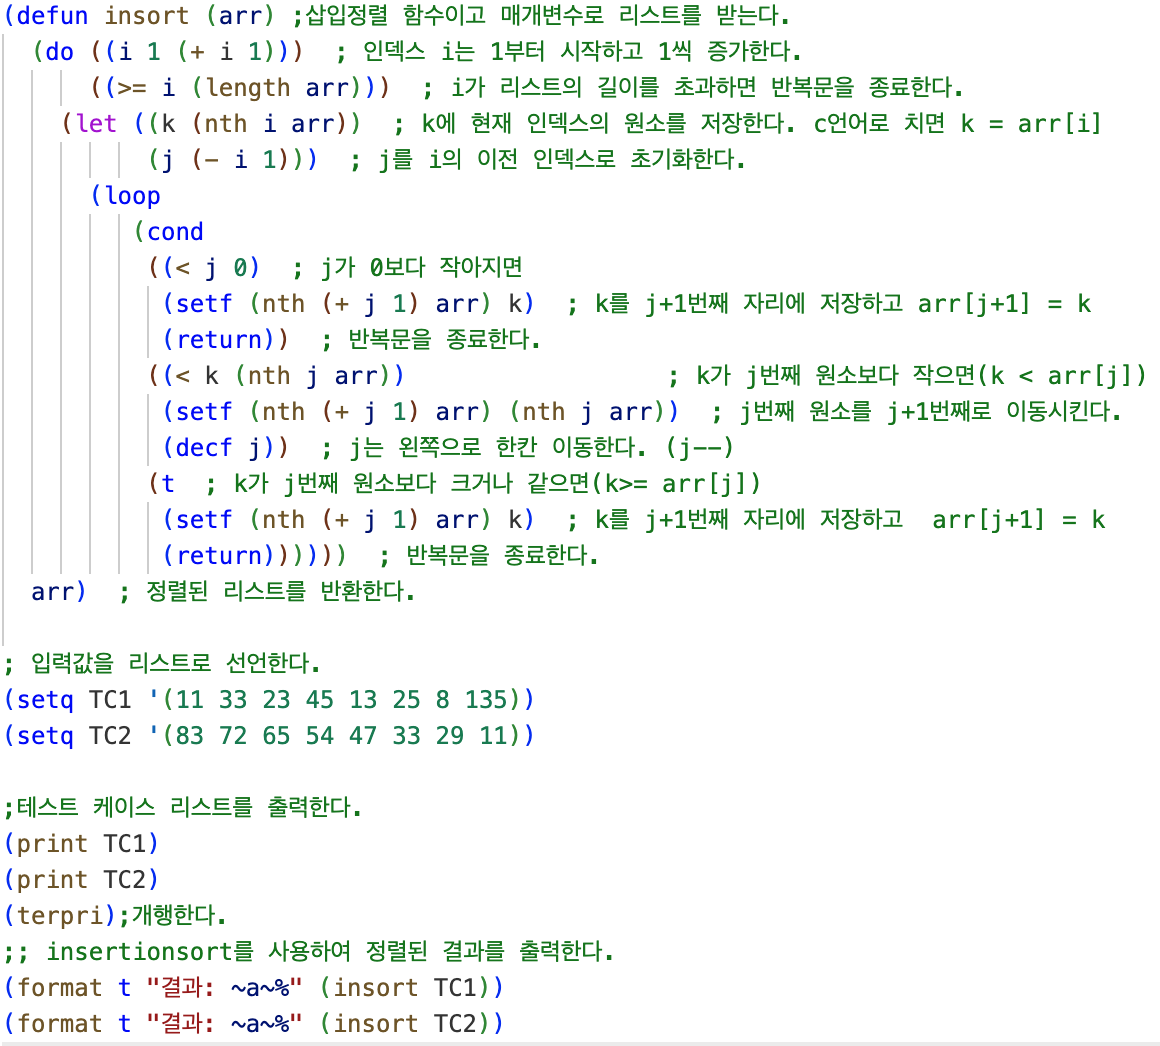
\includegraphics[width = 10cm,height = 6cm]{hw4b_code.png}
    \caption{hw4b 코드}
    \label{fig:fig4}
\end{figure}
\begin{figure}[h]
    \centering
    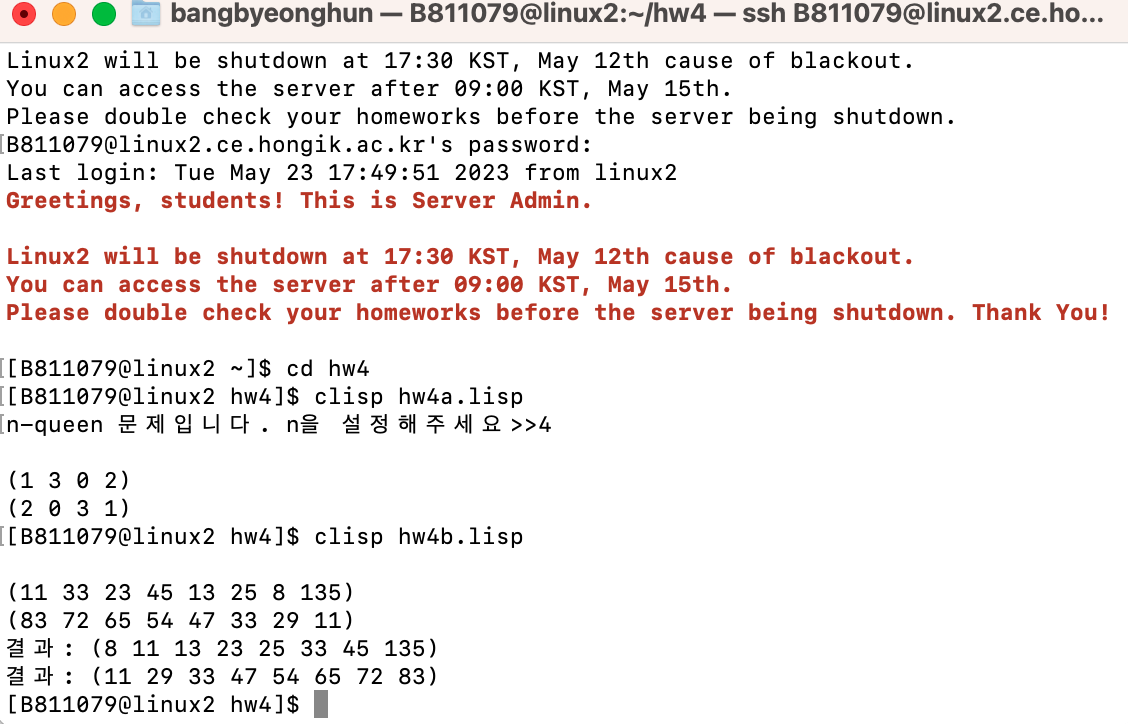
\includegraphics[width = 10cm]{hw4b_run.png}
    \caption{hw4b 실행 결과}
    \label{fig:fig5}
\end{figure}

\end{document}
